\documentclass[12pt, a4paper]{extreport}
\usepackage[utf8]{inputenc}
\usepackage{graphicx}
\usepackage[margin=1in]{geometry}
\usepackage{titlesec, color, blindtext}
\usepackage{titling}
\usepackage{makecell}
\usepackage[
    style=ieee
]{biblatex}
\usepackage[toc]{appendix} % use [page] to include appendix title page
\usepackage{listings}
\usepackage[most]{tcolorbox}
\usepackage{inconsolata}
\usepackage{tabulary}

\definecolor{mygreen}{rgb}{0,0.6,0}
\definecolor{mymauve}{rgb}{0.58,0,0.82}

\newtcblisting[auto counter]{sexylisting}[2][]{sharp corners, 
    fonttitle=\bfseries, colframe=darkgray, colback=white, listing only, 
    listing options={basicstyle=\ttfamily,language=java,morekeywords={export,function,let,await,require},commentstyle=\color{mygreen},keywordstyle=\color{blue},showstringspaces=false}, 
    title=Snippet \thetcbcounter: #2, #1}

\addbibresource{references.bib}
\setlength{\parindent}{1em}
\setlength{\parskip}{1em}
\definecolor{gray75}{gray}{0.75}
\newcommand{\hsp}{\hspace{10pt}}
\titleformat{\chapter}[display]{\Huge\bfseries}{Chapter \thechapter}{0.3em}{\LARGE\bfseries}
\titlespacing*{\chapter}{0cm}{-\topskip}{0pt}[0pt]
\titlespacing*{\section}{0cm}{0cm}{0pt}[0pt]

% \pretitle{
%     \begin{center}
%         \includegraphics[width=\textwidth]{res/universe.jpg}
% 		Department of Computer Science \vspace{0.2cm}
		
% 		Individual Project - CS3IP16
		
% 		\vspace{6cm}
% 		\fontsize{18bp}{18bp}\selectfont
% 	}
% \posttitle{\end{center}}
\title{Using Containers to Isolate Remote Code Execution for an Online Development Environment}
\author{
    Joseph Fazzino\\
    24026478\\
    [4cm]{Supervisor: Dr. Hong Wei}
}
\date{29\textsuperscript{th} April 2019}


\begin{document}

\maketitle
\setcounter{tocdepth}{1}
\tableofcontents
% --------------------------------------------------
% Preamble
% --------------------------------------------------
\pagebreak

% --------------------------------------------------
% Abstract
% --------------------------------------------------
\section{Abstract}
% 250 - 300 words

% outline aims, methods, implementation, achievements, and conclusions

Programming is a skill that has only become more popular in modern times. This project is aiming to replace local tooling that is normally required to start learning with a simple web app that lets users write and execute code without having to install anything. The web app was implemented making heavy use of containers which are used to give every user an isolated environment. This report is a formal write up of the problems being tackled, research that went into the design of the system, different solutions that were explored, implementation of the system, testing of the system and a discussion of the results with speculation for what the future of the project could look like. 

The resulting application created is a fully functioning application with an industry tested code editor, full environment with terminal emulator and educational exercises which can be done and created. The application runs functionally well on all modern browsers and performance testing shows impressive results across both the frontend and the backend. Approaches to mitigating security issues are also covered with a proposal of how to defend against kernel exploits also included.
\pagebreak




\pagebreak

% --------------------------------------------------
% Acknowledgements
% --------------------------------------------------
\section{Acknowledgements}
I'd like to acknowledge Dr. Hong Wei for being my project supervisor. Dan Justin and Dr. Martine Magnan for their continued support through the early stages of my career. Suhail Parmar for contributing to my caffeine levels and providing help with Docker and UNIX. Dan Davis and Max Denning for helping me brainstorm the idea for the project and enduring me talking about frontend for the past year. And finally, my parents, Paul and Joanna Fazzino for being unwaveringly supportive and great role models.
\pagebreak


\pagebreak

% --------------------------------------------------
% Glossary
% --------------------------------------------------
\section{Glossary of Terms and Abbreviations}
The following is a list of abbreviations that are commonly used in this document:

\begin{table}[h]
    \centering
    \begin{tabulary}{\textwidth}{l r}
        \hline
        \hline
        \textbf{Abbreviation} & \textbf{Expansion}\\
        \hline
        \hline
        API & Application Platform Interface\\
        
        CRA & Create React App\\
        
        RTC & Real-Time Communication\\
        
        REPL & Read-Evaluate-Print-Loop\\
        
        REST & Representational State Transfer\\
        
        HCI & Human Computer Interaction\\
        
        HTML & HyperText Markup Language\\
        
        UX & User Experience\\
        
        DX & Developer Experience\\
        
        UI & User Interface\\
        
        JS & JavaScript\\
        
        JSON & JavaScript Object Notation\\
        
        OS & Operating System\\
        
        SPA & Single Page Application\\
        
        P2P & Peer to Peer\\
        
        PaaS & Platform as a Service\\
        
        VM & Virtual Machine\\
        
        VPN & Virtual Private Network\\
        
        LXC & Linux Containers\\
        
        SSR & Server Side Rendering\\
        
        IDE & Integrated Developer Environment\\
        
        CLI & Command Line Interface \\
        
        STDIN & Standard Input\\
        
        STDOUT & Standard Output\\
        
        STDERR & Standard Error\\
        
        TTY & Teletype\\
        
        WS & WebSocket\\
        
        CSS & Cascading StyleSheets\\
        
        DOM & Document Object Model\\
        
        IE & Internet Explorer\\
        
        SEO & Search Engine Optimisation\\
        
        LAN & Local Area Network\\
        
        CPU & Central Processing Unit\\
        
        PHP & Programmers Hate PHP\\
        
        npm & Node Package Manager
    \end{tabulary}
\end{table}
\pagebreak

% --------------------------------------------------
% Table of Contents & Glossary
% --------------------------------------------------



% --------------------------------------------------
% Thesis
% --------------------------------------------------
% --------------------------------------------------
% Introduction
% --------------------------------------------------
\chapter{Introduction}

As computers have become more pervasive, coding has become a skill that has graduated past being something that only people who work in laboratories need to concern themselves with, to a skill that has become highly desirable commercially and is starting to be taught in the regular curriculum to children studying at a primary school level \cite{schools}. This has created a demand for beginner friendly coding tools and environments, this project is proposing to provide a tool to fill this niche by creating an online environment where people can get started with basic coding concepts without having to trawl through documentation and technical detail about how to get running with one of the popular languages/tools available.

This project is attempting to lower the barrier to entry for anyone with an internet connection to be able to get started coding with as little overhead as possible.

\pagebreak


% --------------------------------------------------
% Problem Definition / Technical Specification
% --------------------------------------------------
\chapter{Problem Articulation\\ \& Technical Specification}
% Here you must provide a detailed description of the problem being addressed. 
% This should include a problem statement and description of the context/environment of the problem 
% along with the key stakeholders and their concerns. The problem statement should be succinct 
% and should establish the criteria  by  which  the  problem  would  be  validated  and  accepted  
% as  being  adequately  solved  (i.e. acceptance requirements). 
% A technical specification may be developed against which a range of possible solutions, 
% including the one you implement, can be considered later in your report. 
% Again the PID content should help you when composing this section. You would include an 
% analysis of the situation-as-is. In some cases this may be very simple. 
% In others with socio-technical system contexts it could be complex and require system / architecture  / environment representations 
% (e.g. in algorithms, mathematical models, UML models, XML, ArchiMate models or other means 
% suitable to your domain). You would also include a vision of the situation-to-be where  the  
% problem  is  adequately  solved.  Again  this  might  require  complex  representations.  
% The situation-to-be and its representation should help you when composing the Discussion section.
\section{Context}
As computers have become more pervasive, coding has become a skill that has graduated past being something that only people who work in laboratories need to concern themselves with, to a skill that has become highly desirable commercially and is starting to be taught in the regular curriculum to children studying at a primary level education\cite{schools}. This new demand for beginner friendly coding tools lends itself nicely to the promise of an online based environment where people can get started with basic coding concepts without having to trawl through documentation and technical detail about how to get running with one of the popular languages/tools available. This has led to an explosion of popularity for web applications such as \texttt{codecademy.com} which offer pre-made, executable exercises for a number of languages. A similar platform \texttt{repl.it} offers a more open and free-form experience and attempts to recreate the environment a developer may have on their machine through the web browser along with online compilation.

\section{Problem Statement}
A common pattern with the current platforms that exist is that they provide a strict sandbox within the confines of a predetermined configuration that the user selects, for example, in \texttt{codecademy} and \texttt{repl.it} you're stuck in the environment you pick when you start desired tool. An argument can be made that this makes a new developers life easier as they don't have to consider the more nuanced parts of the file system or learn any sort of terminal commands. However, it seems as though there would be value in a system that can provide both the ease of use that current existing solutions offer and also the freedom to explore a full environment with an array of tools preconfigured that encourage exploration without compromising the security and integrity of the underlying system.

\section{Technical Specification}
The objectives of this project are: 
\begin{enumerate}
    \item Create a platform where users can write/execute code
    \item Give every user their own personal environment
    \item Eliminate the need for locally installed tooling
    \item Provide a system that encourages exploration into the world of development
\end{enumerate}

\subsection{Writing and Executing Code}
\textbf{Functional Requirements}
\begin{itemize}
    \item Code will be able to be typed using the platform
    \item Code will be able to be saved
    \item Code will be able to be read from the platform
    \item Code will be able to be executed
\end{itemize}
\textbf{Non-Functional Requirements}
\begin{itemize}
    \item A good variety of languages will be supported
    \item The basic features of a code editor will be available (i.e. syntax highlighting)
    \item Code that is executing will not stall the platform
\end{itemize}

\subsection{Personal Environments}
\textbf{Functional Requirements}
\begin{itemize}
    \item A personal environment will be allocated to every user
\end{itemize}
\textbf{Non-Functional Requirements}
\begin{itemize}
    \item The personal environments will be isolated from the rest of the system
    \item The personal environments will be isolated from each other
    \item The personal environments will perform well and be responsive to user input
    \item If a personal environment fails then it will be restarted
\end{itemize}

\subsection{Local Tooling Replacement}
\textbf{Functional Requirements}
\begin{itemize}
    \item High quality tools will be available to the user
    \item Industry standard tools will be available to the user
    \item The system will eliminate the need for local tooling
\end{itemize}
\textbf{Non-Functional Requirements}
\begin{itemize}
    \item Popular tools will be researched and considered before being added to the system
    \item Tools will be standardised across the system
    \item Tools will be customisable to the users needs
    \item Tools will behave in a responsive manner
\end{itemize}

\subsection{Encourage Exploration into Development}
\textbf{Functional Requirements}
\begin{itemize}
    \item Implement exercises for users to do
    \item Allow creation of exercises by users
\end{itemize}
\textbf{Non-Functional Requirements}
\begin{itemize}
    \item Allow any exercise to be shared
    \item Assign difficulty level to exercises
    \item Provide an open area for the user to explore their personal environment
\end{itemize}


% --------------------------------------------------
% Literature Review
% --------------------------------------------------
% The literature review is an essential component of your project report. You should discuss the existing literature that is relevant to your project with full and proper referencing. You should aim to refer to a range of material including academic papers, text books, articles and existing product descriptions. It should be clear to the reader why the literature you identify is relevant and how you have incorporated the learnings from your review into your project. For example, you may have made a number of project 
% Page 4 of 5 decisions based on your review of the literature and these decisions should be described. The literature review should also lead to the creation of a number of possible solutions to your problem articulation and technical specification

\chapter{Literature Review} \label{lit}

This chapter focuses on an analysis of existing systems in the online development space and the literature that provides context to the decisions that were made during development. It looks at the advancement of the web browser and discusses the functionality provided which can lead to this type of project to be developed. It also looks at the current state of the art of virtualization as it relates to personalised environments and how the advent of Containers has fundamentally changed the way users interact with virtual environments, as illustrated by supporting literature.

\section{The Web Browser} \label{lit-web}

The web browser has been through a myriad of changes since it's birth in the early 1990s. An excellent article titled "Mosaic and the World-Wide-Web"\cite{mosaic} illustrates the problems that were prominent in the early stages of the industry such as the lack of a search engine leading to difficulty in finding resources. It also illustrates what were considered leaps in progress at the time such as Mosaic being the first browser to support in-line multimedia and to have a 'back' and 'forward' button.

Such concepts that were developed during the time are still very relevant, the general TCP/IP stack had been determined and the HTTP protocol was in use. An issue with HTTP is the protocol by design has latency embedded as it is designed for sending structured messages. For a project attempting to create an environment that mirrors a local set up online latency is a big hurdle and the need for it to be real-time is key. 

\section{Real-Time Communication} \label{lit-web}

An experiment was done in 2012 discussing the performance of different RTC methods by Professors at the University of New Brunswick\cite{websocket}.

\textbf{HTTP polling} is an attempt to solve the real-time issue however it is still built on top of a system not designed for real-time, full duplex communication. \textbf{HTTP long-polling} is another solution that sticks to the HTTP protocol but reduces the number of wasteful requests by having the server intelligently not respond to the request if there is no information available and hang until a timeout or information becomes available.

A modern solution to this is the \textbf{WebSocket} protocol proposed in RFC 6455 \cite{wsrfc} which aims to reduce latency by a factor of 3 compared to HTTP in the real-time communication aspect. It is a fully duplexed, bidirectional communication channel that uses physical sockets to connect machines.

\section{Online Developer Environments} \label{lit-ode}

A number of existing solutions providing online development environments exist and have been analysed for the purpose of this review.

\subsection{Repl.it}
Repl.it is very similar to the idea proposed in the Problem Statement (Section \ref{section:probart-probstate}) and a lot of the requirements lined out in Section \ref{section:probart-techspec}. It offers a huge array of Repl templates available for users to get started with many languages/frameworks very quickly. It also uses the Monaco Editor provided by Microsoft in order to provide a first class text editor experience.

Repl.it takes advantage of containerisation in order to gives users the full developer experience when visiting the system \cite{replit-containers}. The system also uses it's own container orchestration software in order to scale the instances available to users up and down depending on demand.

For long running processes such as a web server. Repl.it will host the process on a subdomain of the repl.it domain which is accessible at any time.

\subsection{Codecademy}
Codecademy is a educational focused online environment designed to teach users how to code. Ranging in topics from beginning web development to a course to the IBM Watson API. It is a more directed experience than Repl.it as users are performing tasks for exercises but they are typing code into a similar environment, the code is executed and the result is displayed to the user.



\subsection{Glitch}

\section{Containerisation and Virtualisation} \label{lit-containers}

https://ieeexplore.ieee.org/abstract/document/6903537

^^ Talking about containers vs VMs for PaaS software

https://ieeexplore.ieee.org/abstract/document/7158965

^^ More focused on Docker

\pagebreak


% --------------------------------------------------
% Method
% --------------------------------------------------
\chapter{The Solution Approach} \label{solapp}
% Here you should identify and evaluate the solution options against your problem statement / technical specification and make a reasoned choice of your chosen solution approach. Why did you do what you did? Conclude with a succinct definition of your solution approach and criteria by which the solution would be accepted as adequately verified. It is very likely that you will add further reference material in this section.

\section{Solutions for Environment Virtualisation} \label{subapp-virt}
In order to provide users with the most 'local' experience as possible on a remote platform it is key to analyse various technologies and techniques that are currently in widespread use in the industry. As discussed during Chapter \ref{lit} there is an consensus in the industry that containers are the better solution for PaaS type software of which this project would fall into the category of.

There are many different container solutions available currently, many have similar roots such as a backbone of using LXC but they build on top of those foundations in varying ways. Some of these ways are documented in the paper which was discussed in Section \ref{lit-containers} \cite{contsvsvirt}. This paper performed a comparison of the various different container technologies and stacked them against each other on key implementation features such as performance and security.

The decision to not research Virtual Machines as a potential solution for the system is due to the project not requiring the utility of a hypervisor. As almost all developer tools are freely available through most Linux distributions. This means that there are few to no downsides of using a container based solution versus a fully blown Virtual Machine set up and many benefits.

\subsection{Container Providers} 

A big limitation of OpenVZ is that it can't run on the standard Linux kernel so it is not a very viable solution for this project as the aim to to deploy the system and requiring a modified kernel will add complexity.

\subsection{Virtualisation Conclusion}

For the system, Docker seems to be the clear choice as it provides good tooling with its daemon. A strong foundation on top of LXC, and it doesn't require additional modification before it can be used on a computer/server which is preferable to avoid for this project.

\section{Chosen Solution for Real-Time Communication} \label{solapp-rtc}

Based off the research performed in Section \ref{lit-rtc} it would seem as though WebSockets fit the requirement of the project in order to ensure rapid communication between the client and their virtual development environment.

By using WebSockets it will be possible to have incredibly low latency bidirectional messages sent from the client to the server which can give the server instructions on what to do with the container that the client is allocated. The ability to send structured data chunks in string form makes it perfect for sending code and returning the output that is executed by the container.

WebSockets are available through the native Web APIs and so no 3rd party dependency is required to interact with them on the client side.

On the server side there are a few ways to implement a WebSocket endpoint but as Node.js and Express are already being used for the REST api it using a 3rd party dependency such as \texttt{express-ws} makes the most sense.

\section{Requirements for Frontend} \label{solapp-frontend}

In order to create an experience that emulates a local installation of tooling and a text editor it is necessary to make sure that a tooling solution is chosen for this project that can meet these needs. The key requirements for the user facing side of this project are:

\begin{enumerate}
  \item Text Editor with essential features that users expect in a standard developer environment
  \item A terminal emulator that can display output of code to users and allow input where it is appropriate
\end{enumerate}

Without these two features there is no way to adequately provide users with an environment that can be anywhere near the level of quality that they would expect from a local installation of tools.

\subsection{Text Editor}

A text editor is a vital part of a developers tool-chain and a few solutions exist on that can be rendered in the web browser. The reason a simple text input cant be used is that a text editor performs actions such as automatic indentation which, while could be recreated, is very specific to languages where for some indentation doesn't matter and for some it is how the language detects what code belongs to what block or function.

With this in mind it is helpful to establish a list of features that are a key requirement for any text editor.

\begin{itemize}
  \item Automatic indentation
  \item Syntax colouring
  \item Control + F compatibility for Find
  \item Bracket matching
  \item Copy-Paste compatibility
\end{itemize}

With these features in mind it is now worth investigating the available resources to see which one satisfies the features best and if any bonus features cna be found.

\subsubsection{Ace - \textit{https://ace.c9.io/}}

Ace is a code editor which is used by Amazon in order to provided their cloud based IDE 'Cloud9' it offers all the features that are listed above and notably includes support for themes, multiple cursors and bracket highlighting.

It's worth noting that Ace is first and foremost a code editor for online use and isn't available for users to install locally.

\subsubsection{CodeMirror - \textit{https://codemirror.net/}}

CodeMirror is another code editor that is exclusive to the browser, it is the code editor that both Firefox, Chrome and Safari use inside their dev tools. It offers all the same features as Ace, however it has a more modern design which more accurately resembles a locally installed text editor.

CodeMirror claims to have experimental support for mobile browsers however it isn't an experience that is good enough to consider as a bonus feature for the editor.

\subsubsection{Monaco - \textit{https://microsoft.github.io/monaco-editor/index.html}}

The Monaco text editor is made by Microsoft and used in their very popular code editor 'VSCode'. VSCode is one of the most popular text editors at the moment for a variety of different developer communities such as web developers and people starting out with a new language that don't want to have to deal with a fully blown IDE.

Feature-wise it offers all the features that are offered by CodeMirror and Ace but also comes built in with auto complete support for TypeScript, JavaScript, HTML and CSS. Through language servers as well, any language can gain support for auto complete for the standard language syntax. It also comes with a 'diff-editor' mode which can be used to gently introduce users to the idea of version control.

Monaco does not have as many themes available as the alternatives but the features that it does offer outweighs the value that alternate themes provides.

\subsubsection{Decision on Text Editor}

Based on the details above it makes a huge amount of sense to use the \textbf{Monaco Editor}, being provided by Microsoft is a significant benefit and the fact that it powers one of the most popular code editors that is being used in the industry means that it will provide as close an experience to a local coding environment as any of the other options.

Giving users experience with this tool will mean the transition to local development tools will be less abrasive as they already know the features that are available in these industry tools. The ability to provide auto complete for some languages is a huge benefit as well as new developers can be sure that the syntax they write is correct.

\subsection{Xterm.js Terminal Emulator - https://xtermjs.org/}

For online emulation of a terminal/command line the most popular solution is \textbf{Xterm.js} which has widespread adoption across many developer tools that require emulation of a terminal. It is used with VSCode in order to give users access to their local shell. It is highly performance focused in order to provide low to no latency between keystrokes and when they render on the screen. It also provides an array of addons that mean the terminal can be connected to a WebSocket stream so the online terminal can be connected to a real terminal on a machine. This is a key feature of a local development environment and therefore Xterm.js is ideal for this project.

\section{Solution for Building the Interface} \label{solapp-tools}

With the solutions established above it is now appropriate to evaluate the options when it comes to how to build the whole user facing side of the system.

As the developer has the most experience building websites using the \texttt{React} library (https://reactjs.org/) to help with creating reactive, data driven, single page web applications, that is the overarching technology that will be used to build the solution.

Within the React ecosystem however, there is a number of options about how to manage certain essential features such as page routing and how to style components in a way that fits into the React methodology.

\subsection{React Framework Options}

In order to get started with React the recommended way is to use a package called \texttt{create-react-app} however a limitation of this method is that it is not configurable to the extent that is required by the Monaco code editor if syntax colouring is considered a key feature, which it is.

It is necessary then to evaluate some other options for getting started with a React application that allows for the configuration options that means syntax colouring works.

The popular options in the community are: ejecting a CRA project, Next.js or Razzle.

\subsubsection{Eject Create-React-App}
Ejecting a CRA provides the developer with full access to all the configuration options that are previously abstracted away. It also installs a lot of dependencies that need to be maintained correctly and the configurable options are overwhelming when all that's required is a few lines added to a config file. This solution is undesirable.

\subsubsection{Next.js - https://nextjs.org/}
Next.js advertises itself as a React 'framework' as it provides many additional features out of the box versus traditional CRA projects. It offers functionality for:

\begin{itemize}
  \item Routing via the File System
  \item Code Splitting
  \item Server Side Rendering
  \item High Level Configuration
\end{itemize}

With these features, fewer external dependencies are required and the configuration which is needed to get syntax colourisation working is available.

\subsubsection{Razzle - https://github.com/jaredpalmer/razzle}

Razzle attempts to find a middle ground between the opinionated decisions made by Next.js and the overwhelming amount of configuration that is required after ejecting an app created by CRA. It is also agnostic to the technology that you use it with so it can be used with several other different frontend libraries such as \textit{Vue.js}.

Due to the less opinionated nature of the project the only real benefit provided by it is the server side rendering and configuration options that is also provided by Next.js.

Despite similar configuration extensibility as Next.js trying to enable syntax colouring for the Monaco editor didn't work.

\subsection{Conclusion on Frontend Framework}

As syntax colouring has been described as a key feature there isn't much of a choice beyond choosing to use either Next.js or the Ejected CRA. As Next.js has a number of other benefits however, this makes it the most attractive and powerful option for building the frontend.

\section{Design Prototypes} \label{solapp-design}

Trying to build a system that provides users with an environment where they feel as though there's not a high barrier to entry involves a design process which has to ensure that things are arranged in as friendly a way as possible.

Some sketches were done in order to try to narrow down what kind of design language should be used to give the users a sense of friendless versus the more stark, professional look that some developer focused websites aim for \texttt{StackOverflow dot com}. Based on these general requirements the following low fidelity prototypes were created presenting different ways that information could be displayed for users.

\begin{figure}[!htb]
  \minipage{0.32\textwidth}
  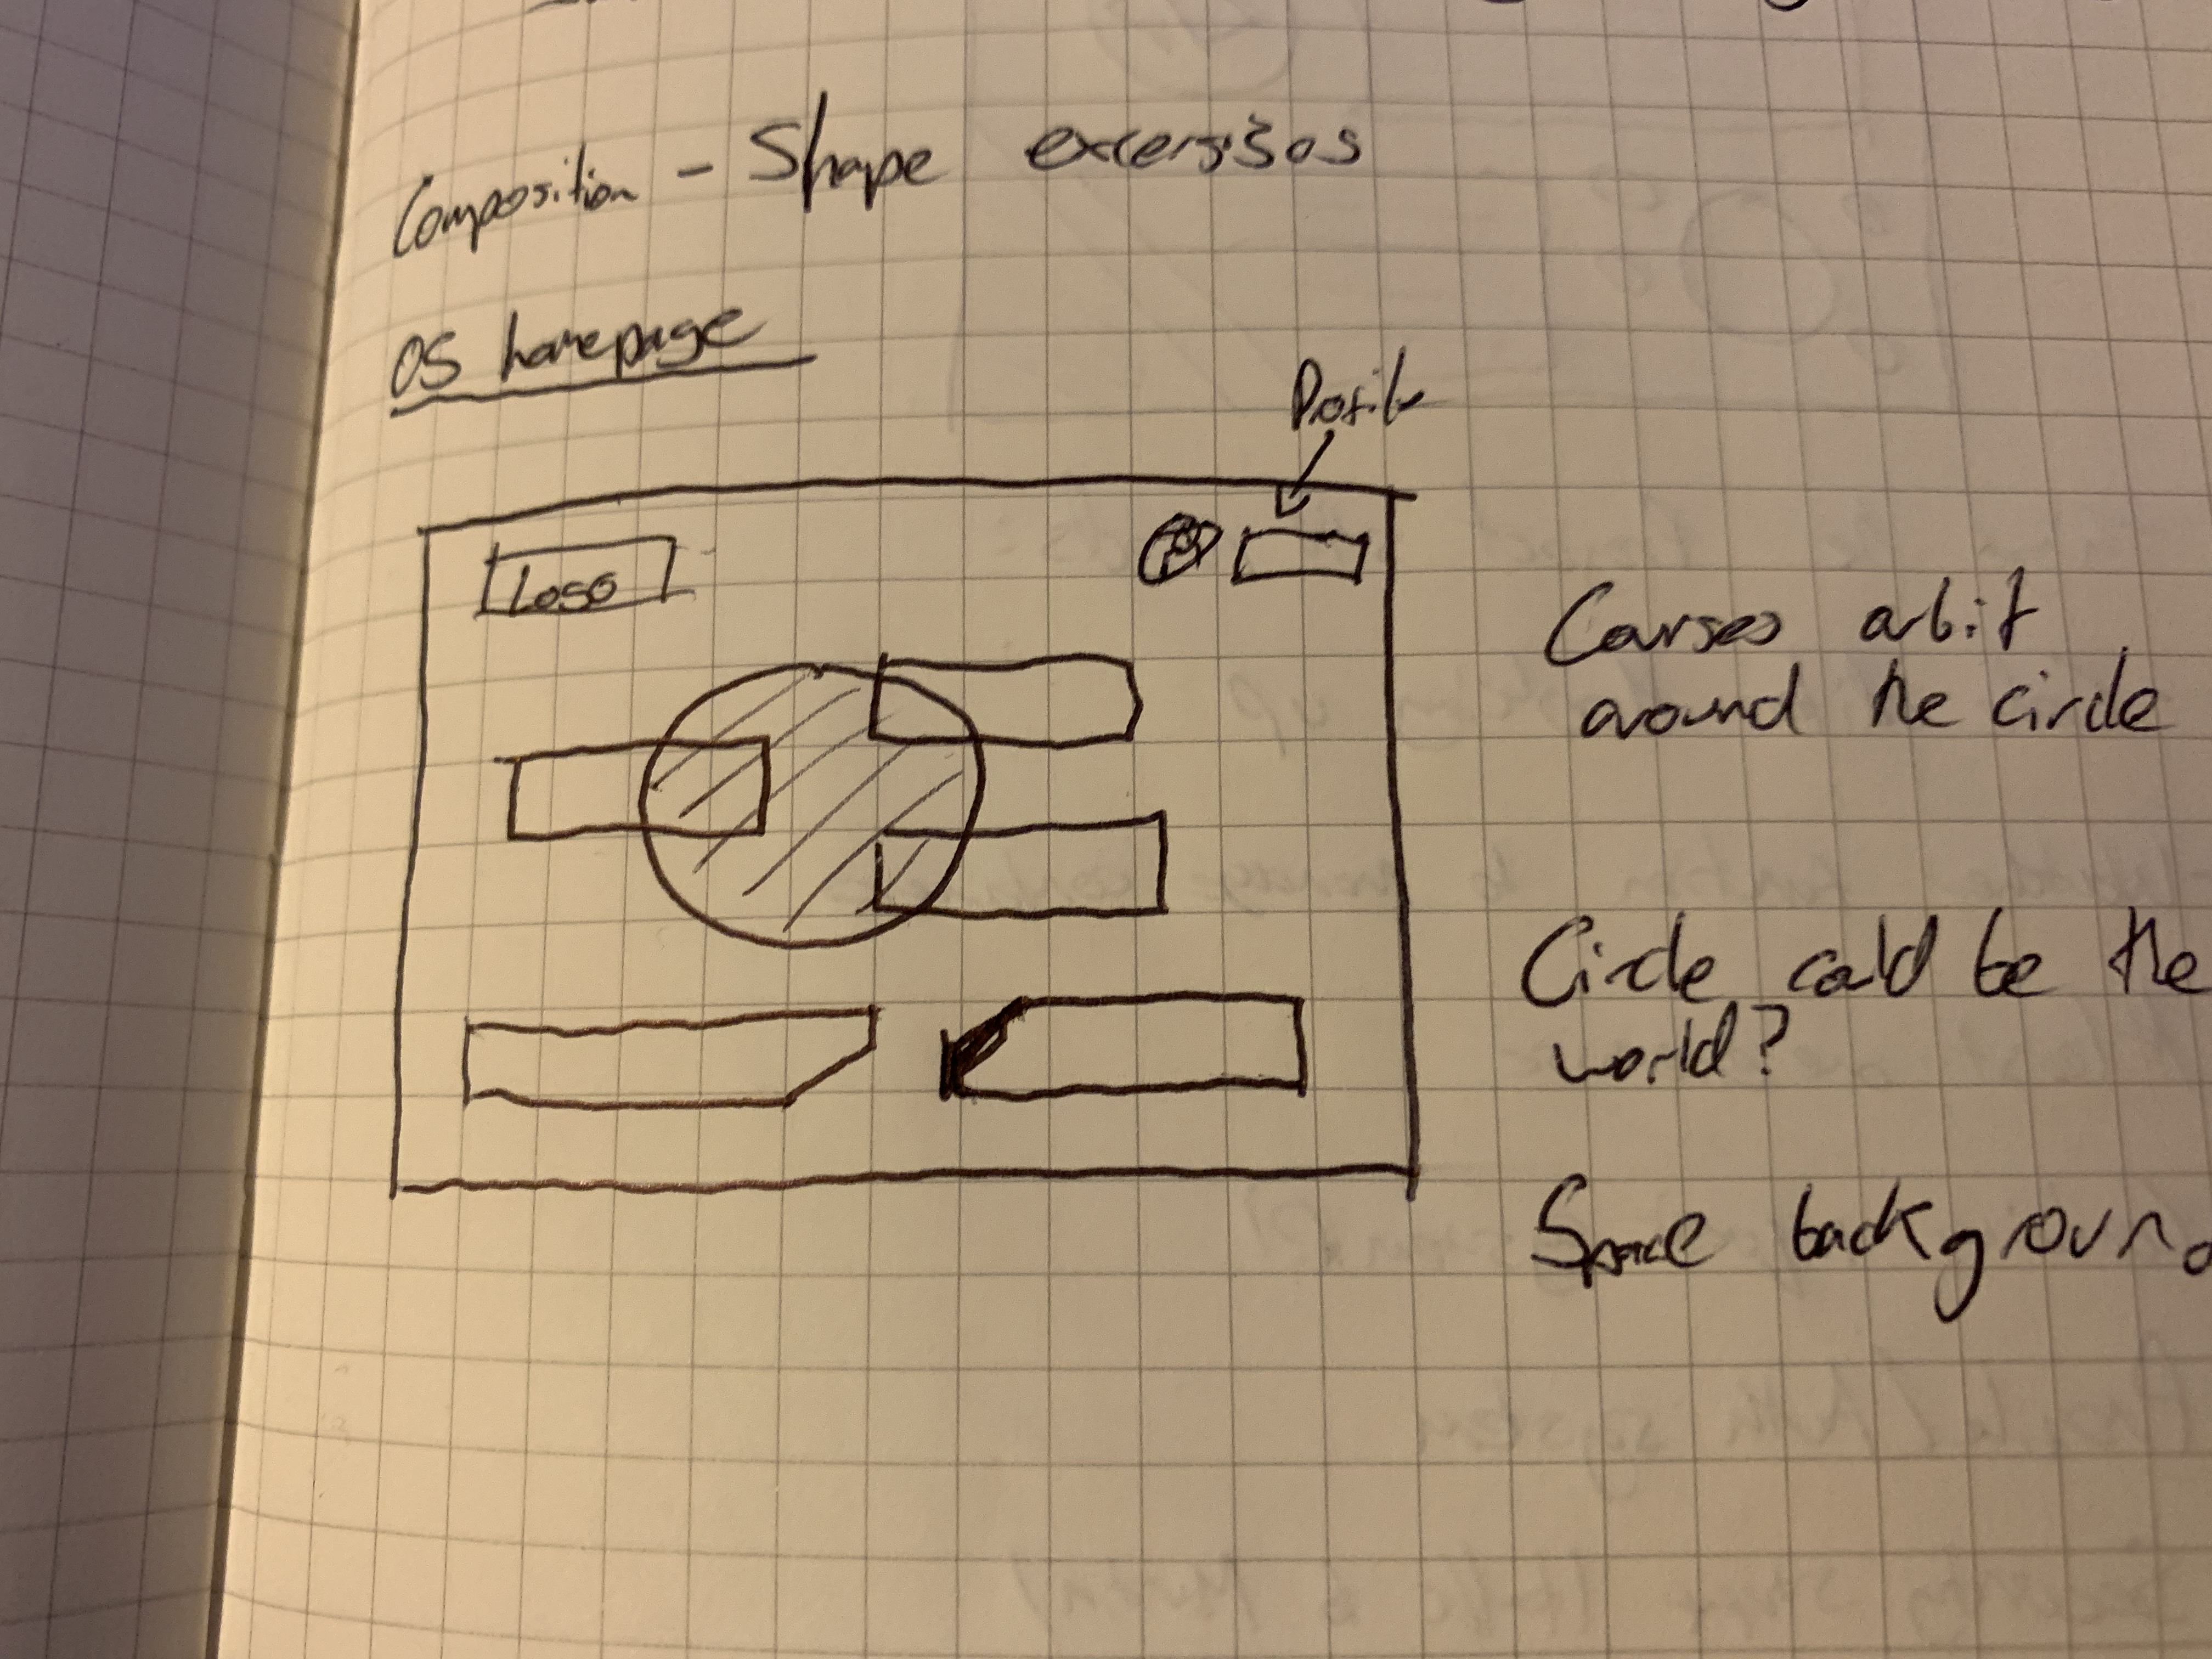
\includegraphics[width=\linewidth]{res/lofi-prototype-1.jpg}
  \caption{Prototype 1}\label{fig:lofi-prototype-1}
  \endminipage\hfill
  \minipage{0.32\textwidth}
  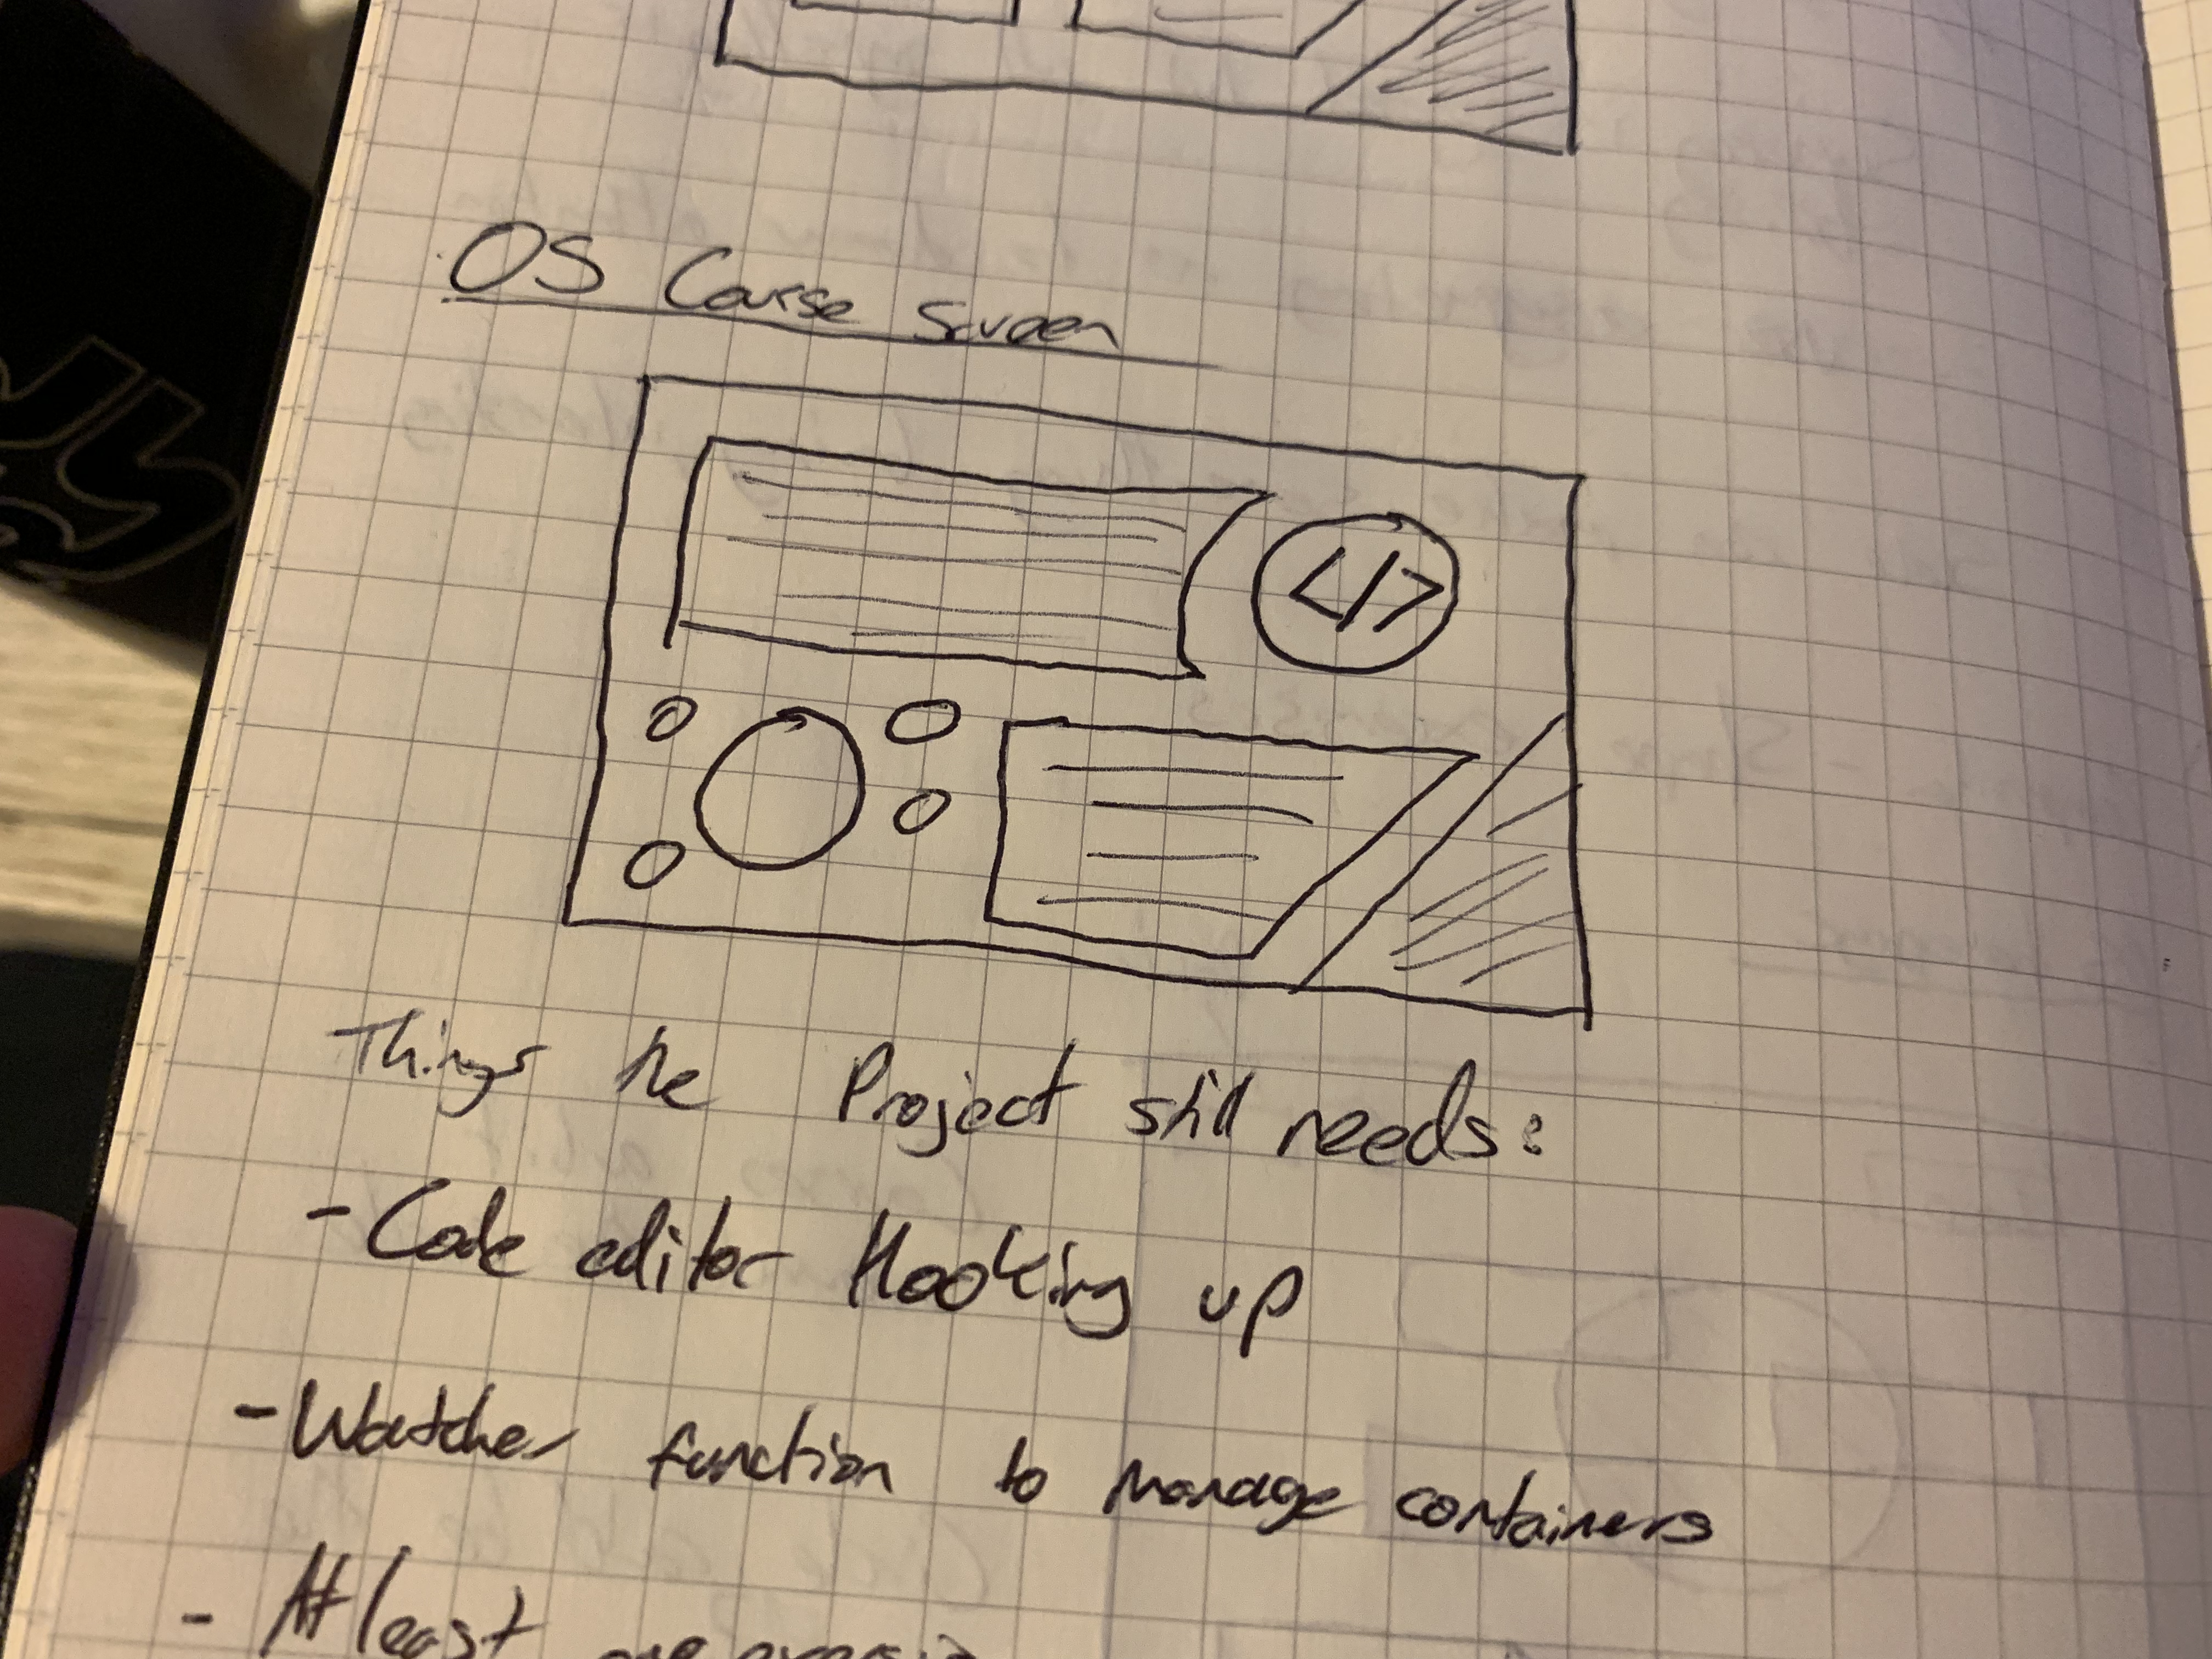
\includegraphics[width=\linewidth]{res/lofi-prototype-2.jpg}
  \caption{Prototype 2}\label{fig:lofi-prototype-2}
  \endminipage\hfill
  \minipage{0.32\textwidth}
  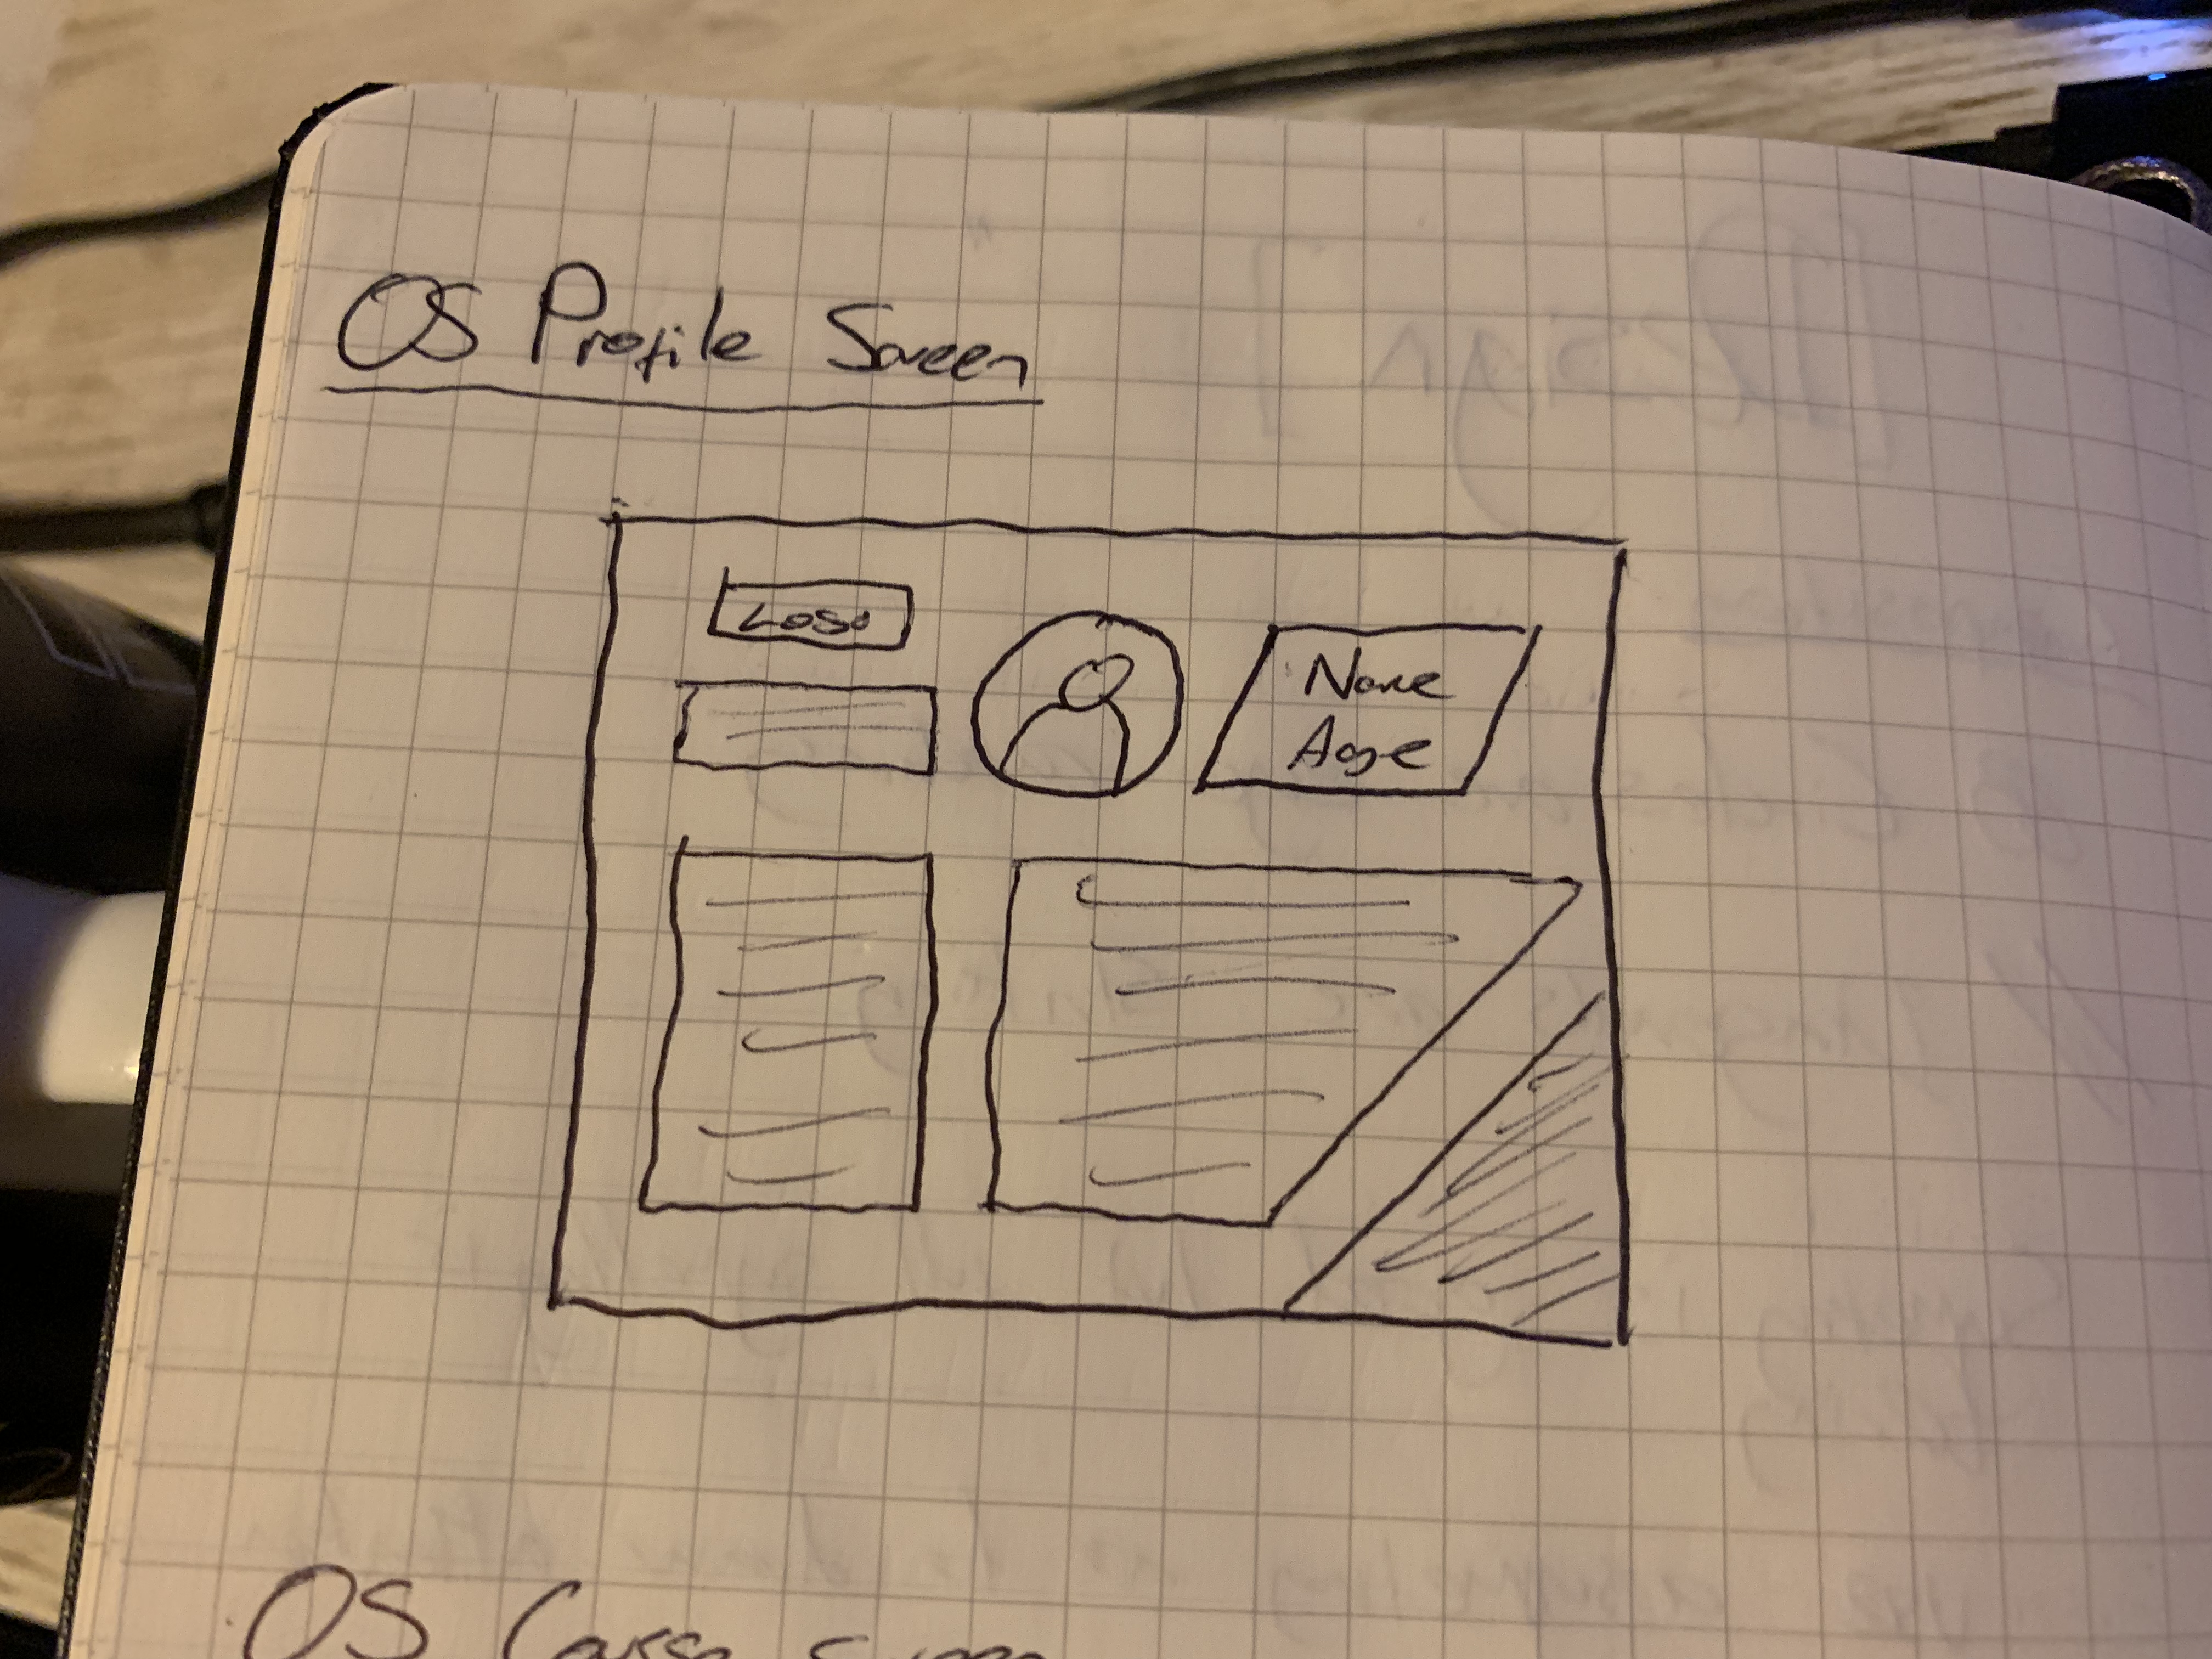
\includegraphics[width=\linewidth]{res/lofi-prototype-3.jpg}
  \caption{Prototype 3}\label{fig:lofi-prototype-3}
  \endminipage
\end{figure}

\subsection{Prototype One}

Prototype design one uses small blocks of informative text which orbit around a circular shape in the middle. Not having significantly large blocks of text means the user won't be intimidated by the information being displayed to them.

The circle is a technique that designers use in order to draw the viewers attention to a specific area. Although it is not shown in the prototype image the font styles that are in use are: one serif font for the display text (the titles and headings) and one sans serif font for the body text (bulk of text).

Some navigation elements can be seen along the top representing different sections of the site.

\subsection{Prototype Two}

Design two uses circles in the same way that prototype one does in order to draw users attention however it also uses interesting borders and shape cut offs to make the website stand out against most websites which stick with the default rectangular shape of most UI elements.

This prototype contains a lot of textual information and might be more relevant for a page that needs to convey a message to the reader that requires significant blocks of text. This design wouldn't be appropriate for a landing page but maybe would for a page on an exercise the user can do.

The font styles in use are a \texttt{monospaced} font for the display text and a sans serif font for body text.

\subsection{Prototype Three}

The third design is a concept for a profile screen but could be applied to a page that represents a particular language and technology. It has lots of space for informative textual content as well as some space for image assets/other resources that might convey information in a less traditional method.

It attempts to use more shapes in order to draw attention to certain areas of the page although it does give the page a slightly skewed look on the right hand side so perhaps if this design were to be implemented it may not render on the screen in a way that looks good.

No specific font styles were decided upon for this prototype.

\section{Overall declaration of solution chosen}

Based off of the research conducted in Chapter \ref{lit} and the potential woes of implementing some of the solutions proposed in this chapter. The current solution approach for creating a full implementation of the system is to have a Next.js frontend with a backend that uses Docker containers in order to implement virtual environments for users. The frontend will make use of the Monaco code editor and the Xterm terminal emulator. Communication between the containers and the frontend will be done with the WebSockets RTC method.

% TODO: put a diagram of the overall structure here (low level)

% TODO: talk about backend stuff here as well :(

\pagebreak


% --------------------------------------------------
% Implementation
% --------------------------------------------------
\chapter{Implementation}

% Here you describe the detailed design of your solution and the details of the actual implementation. It may be appropriate to discuss aspects of design or implementation that were particularly problematic and/or novel. This section may well be one of the largest in your report and the exact contents will be unique to your project and so there are no general guidelines. Use of several sub-sections here is appropriate.

This chapter focuses on the overall implementation of the system and walks through how the separate components interface together and interact in a way that provides the user with a positive experience.

\section{Back-end}

The back-end of the system is implemented in Node.js and provides the API that the front-end will interact with through REST requests and WebSocket messages. TypeScript \cite{typescript} is being used rather than plain JavaScript in order to provide support for static types and catch more errors during the build time compilation rather than during run time.

A link to the back-end code can be found in Appendix C

\subsection{Database}

The database use MongoDB \cite{mongo}with two collections, one for exercises and one for activities. An exercise can have many activities but activities can only belong to one exercise.


For the Node server to be able to make database calls the MongoDB API must be used. This is done via the \texttt{mongoose} package \cite{mongoose}.

\subsection{REST API} \label{impl-rest}

To provide an API that a front-end can interact with to retrieve information from the database, a REST API is created with the Express framework \cite{express}. Creating an API endpoint with Express is a simple process that follows the formula of:

\texttt{AppObject.RequestType("Endpoint", CallbackFunction)}

Where \textit{AppObject} is the variable representing the instance of the server. \textit{RequestType} is usually one of GET or POST (HTTP verbs). \textit{Endpoint} is a string representing the local path the handles the request and \textit{CallbackFunction} is the function that handles the request and sends the response.

The code \texttt{app.get("/profile", callback)} is the function that handles GET requests to the \textbf{/profile} endpoint. 

The only REST endpoints in the back-end code are related to the exercises section of the system as those need to be stored in a global database. Most of the communication between the front and back is implemented through WebSocket connections.

\subsubsection{Get Exercise Endpoint}

The \textbf{/exercise} endpoint is a GET request that returns the related exercise in the database that corresponds with the ID that is sent along in the query string.

The callback function that deals with the request and sends a response is shown for this endpoint and it sends a HTTP Status Code 404 if it can't find the exercise based on the ID passed in the request and a HTTP Status Code 500 if there was an error with processing the request (such as if the database is down). Otherwise it will send a HTTP Status Code 200 and the exercise JSON object.

\begin{sexylisting}{/exercise endpoint}
server.get("/exercise", (req: Request, res: Response) => {
    const { id } = req.query;

    Exercise.findById(id)
        .populate("activities")
        .exec()
        .then(exercise => {
            if (exercise) {
                res.send(exercise);
                return;
            }
            res.sendStatus(404);
        })
        .catch(err => {
            res.status(500).json(err);
        });
});
\end{sexylisting}

\subsubsection{Create Exercise Endpoint}

The \textbf{/create} endpoint is a POST request used when a user makes a new exercise. Here the request object is broken down to get the parameters sent with the request and is turned into objects that can be inserted into the database.

The response is the endpoint that the front-end can use to navigate to the page for the newly generated exercise.

\begin{sexylisting}{/create endpoint}
server.post("/create", (req, res) => {
    const { activities, title, description, language } 
        = req.body;

    console.log(req.body);
    const acts = activities as IActivity[];
    
    {...}
});
\end{sexylisting}

\subsection{Docker Integration} \label{impl-docker}

For the back-end to have the ability to create and link Docker containers to a user running the application on the front-end it needs to be able to interact with the \textit{Docker Socket}. Every machine with an installation of the Docker Engine has a Docker Socket which is what the Docker CLI uses when commands are run against it.

There is a popular package on NPM called \textbf{Dockerode} \cite{dockerode} which enables interaction with the Docker API via whatever socket/path is provided in it's configuration.

The following code snippet shows the instantiation of the Dockerode package using the local Docker socket and exports it for use in other files in the project's back-end.

\begin{sexylisting}{Create Docker instance and point it to local Socket}    
import Docker = require("dockerode");
const SOCKET_PATH = "/var/run/docker.sock";
const options = { socketPath: SOCKET_PATH };
export default new Docker(options);
\end{sexylisting}

\subsubsection{Provisioning a User Allocated Container} \label{impl-alloc}

Creating a container for every user that connects to the system requires the concept of a \textit{basic image}. This image is created from a Dockerfile which specifies the defaults for all user's environments. The Dockerfile is responsible for configuring the environment so that it is secure and pre-installed with all the tools that the user might need.

The basic image comes with the following software pre-installed: \textbf{Alpine Linux Distro}, \textbf{Bash}, \textbf{Python3}, \textbf{Node.js}, \textbf{GCC} and \textbf{Git}.

Alpine Linux is the distribution that the base image of the container is based on. Bash is a very common shell which is a better default than the standard \textit{ash} or \textit{sh} shells which come with the Alpine image. Bash is important for the code execution aspect of the system which is explained further in \textit{Executing Code - \ref{imp-execode}}. Python, Node and GCC are chosen as those are the three runtimes that are supported by the system. Git is installed so if the user develops something that they want to be able to save they can access Git through the command line.

% TODO: Ref the dockerfile in the appendix
Some additional configuration that is done in the Dockerfile is the creation of the user account that users of the system will be operating as while they're connected to the container. By default the Docker engine sets the user of a container as root but this is not appropriate for a system where anyone can play with a container so a low permission user is created called \textit{damien} who has their own home folder and ownership of that folder but everything under the root directory is protected.

The JavaScript to create the container for the user is a simple function call referencing the Docker API variable.

\begin{sexylisting}{Create container with options}
const container = await docker.createContainer({
    Image: "basic",
    AttachStdin: true,
    AttachStdout: true,
    AttachStderr: true,
    Tty: true,
    Cmd: ["/bin/bash"],
    OpenStdin: true,
    StdinOnce: false,
    name
});
\end{sexylisting}

This tells the API to create a container using the image with the label "basic" which is the label of the image created from the Dockerfile. The \texttt{AttachX} properties tell the container if they should allow other processes to attach to this containers Standard Input/Output/Error which, as this container is emulated on the front end, are required to be \texttt{true}. \texttt{Tty} refers to a way of referring to the interface for a terminal. Without this option set to true it won't display in a way that looks like a traditional command line environment. \texttt{Cmd} is the command that the container should run once it's been created, in this case it needs to run bash. \texttt{OpenStdin} allows standard input to the TTY. \texttt{StdinOnce} will close the STDIN connection if an attached user disconnects, this needs to be off for this system as going between an exercise and a container will detach in the way that satisfies this requirement and it needs to be able to reconnect to the STDIN. The \texttt{name} property is the labelled name of the container which is displayed to the user when they connect.

\subsubsection{Provisioning an Exercise Container} \label{impl-exer-cont}

Provisioning the exercise container is similar as the user's allocated container but it has to pause the allocated container so that resources aren't being wasted and then create the container for the exercise.

Exercise containers are created when a user enters an exercise and are destroyed when a user leaves the exercise. The are created the same way with the same configuration as the allocated containers however the image they are based on is the simplest REPL image that exists that relates to the runtime that the exercise is for.

\subsubsection{Executing Code} \label{imp-execode}

Getting code from the server to inside a file on the container and then executing is a fundamental requirement of this project and is achieved by taking advantage of Bash which is configured to come on every container created by the system.

The execute command in Docker (exec) is only capable of running a single command with arguments. In Bash however there is a way of chaining commands as arguments using the \textbf{-c} option. A JavaScript function called \texttt{getCodeSaveCommand} creates the command that the Docker execute command can run in order to save the file.

\begin{sexylisting}{Create command to save code to container}
export function getCodeSaveCommand(filename, code) {
    let cmd = ["/bin/bash", "-c"];

    code = code.replace(/`/g, "\\`");

    cmd.push(`echo "${code}" > ${filename}`);

    return cmd;
}
\end{sexylisting}

This snippet will add an escape character in front of all double quotes so that the double quotes don't finish the \texttt{bash -c} command and add command that saves the code to the specified file to the cmd array. This array is what the CMD option accepts. 

After the file has been saved successfully a message is sent to the client confirming the save and the client sends an attach request for the code execution so that STDIN and STDOUT can be attached to the terminal emulator.

The execute command to run the code is more straightforward than the command to save it to a file.

\begin{sexylisting}{Creating the code execution command for the container}
export function getCodeExecutionCommand(filename, repl) {
    let cmd = ["/bin/bash", "-c"];
    
    if (repl === Repl.C) {
        return cmd.concat(
            `gcc ${filename} && ./a.out && rm a.out`
        );
    } else {
        return cmd.concat(
            `${repl} ${filename}`
        );
    }
}
\end{sexylisting}

This snippet works similarly the same lines as the previous however more steps are involved for the C compilation step as an output file is generated which has to be executed.

\subsection{WebSockets - Back-end} \label{impl-ws-back-end}

As mentioned in the Solution Approach (Section \ref{solapp-rtc}), the standard WebSocket client is available as a browser API and on the back-end a middleware package \texttt{express-ws} \cite{expressws} is being used to allow connections to the server using the WebSocket protocol.

\subsubsection{Endpoint Configuration} \label{impl-ws-config}

For the server to be able to create a WebSocket connection with clients and endpoint must be created that accepts the WebSocket protocol. 

\begin{sexylisting}{Setup of WebSocket Endpoint}
    server.ws("/", (ws: WebSocket) => {
        console.log("Connection Made");
        startBasicContainer(ws)
        {...}
    }
\end{sexylisting}

The snippet above shows that a WebSocket connection can be made to the root endpoint of the server and once the connection is made it is logged to the console and the function to create the basic user allocated container is called.

\subsubsection{Message Structure} \label{impl-ws-msg-struct}

WebSockets are only capable of sending strings of text in their messages however, as JSON is a way of representing objects through strings a template message guide can be created.

\begin{sexylisting}[label={code:ws-msg}]{WS message}
    const message = {
        type: MessageTypes.CONTAINER_STOP,
        data: { id }
    };

    socket.send(JSON.stringify(message));
\end{sexylisting}

This snippet shows an example message which is a JSON object with two properties \texttt{type}, which represents the type of the message being sent, and \texttt{data} which is an object itself which contains any relevant information that might be useful for the other end of the socket. In this case the type of the message is a flag to stop a running container and the data is the ID of the container. This is sent after being stringify-ed by the built in JSON object.

\subsubsection{Message Types} \label{impl-ws-msg-type}

As can be seen above each message has a type. These types are processed through a \texttt{switch statement} which inspects the type, extracts the parameters from the \texttt{data} property and makes a function call.

\begin{sexylisting}{How the messages are processed by the back-end}
    const { type, data } = JSON.parse(msg);
    switch (type) {
        case "Container.Pause":
            // Used when focus is lost from tab
            console.log("Pausing container");
            stopContainer(ws, data.id);
            break;
        case "Container.Resume":
            // Used when focus is resumed via tab
            console.log("Resuming container");
            resumeContainer(ws, data.id);
            break;
        {...}
\end{sexylisting}

The first thing done when the message is received is to parse it into JavaScript objects and the \texttt{type} and \texttt{data} properties are extracted. The \texttt{type} is switched against and based on what the value of it is. A string is logged to the console showing what action the server is performing and a function is called which will always pass the WebSocket object (so the server can reply) and then passes any relevant data that is required by that function. 

\subsubsection{WebSocket Streams} \label{impl-ws-streams}

Streams is a concept in programming which directly means a \textit{stream of data}. Streams are used most often to act on a huge amount of data in a more performance focused way. Streams of events are the types of streams that are used in this project as the Docker containers are able to stream their STDIN and STDOUT. Using the Node.js Stream API it is possible to \texttt{pipe()} these streams over WebSockets.

The package \texttt{websocket-stream} is used in the server to enable the streams to be piped over the WebSocket connection.

\begin{sexylisting}{Endpoint which connects the container stream to the WebSocket}
server.ws("/connect", (ws: WebSocket, req: Request) => {
    const stream = websocketStream(ws, { binary: true });
    console.log("Trying to connect streams");

    attachSocketToContainer(
        stream,
        req.query.id,
        req.query.bidirectional,
        req.query.logs
    );
});
\end{sexylisting}

This snippet shows that a WebSocket connection can be opened to the \texttt{/connect} endpoint of the server where a stream will be created from the WebSocket. When the connection is made a function is called to attach the WebSocket stream to the container stream and it passes the stream created by the websocket-stream package, the id of the container to attach the stream to, whether the stream is bidirectional (allows STDIN and STDOUT) and if the previous logs from the container should be allowed.

Streams are a core concept in Node.js so passing one stream to another is simple.

\begin{sexylisting}{Attachment of the container stream to the WebSocket stream}
container.attach(
    {
        stream: true,
        stdout: true,
        stderr: true,
        stdin: isBidirectional,
        logs: showLogs
    },
    function(err: Error, stream) {
        {Error Handling here...}
        console.log("Stream Connection Established!");
        if (isBidirectional) {
            stream.pipe(wss);
            wss.pipe(stream);
        } else {
            stream.pipe(wss);
        }
    }
);
\end{sexylisting}

The snippet above is showing the Docker API making a call to attach to the running container that was calculated based on the ID passed to the function. The options show that the \texttt{stream} option is set to true, the \texttt{stdin} option is dependent on if the stream is set to be bidirectional or not and the \texttt{logs} are also determined by the parameter passed from the query string.

The callback function does error handling and then will pipe the container stream to the WebSocket stream. If bidirectional flow is enabled, it will also pipe the WebSocket stream to the container. 


\section{Front-end}

The general approach for developing the front-end of the project is stated in Chapter \ref{solapp} in Section \ref{solapp-front-end} but a number of other packages were used to make the development of the solution smoother and less error prone. Namely, TypeScript \cite{typescript} was used rather than plain JavaScript and Styled Components \cite{styledcomp} was used in addition to regular CSS to make implementing the design more straightforward.

The front-end consists of 4 pages or screens all of which have varying degrees of functionality and interaction with both the back-end and the user.

A link to the front-end code can be found in Appendix C.

\subsection{WebSockets - Front-end} \label{impl-ws-front-end}

The WebSocket configuration is similar to the back-end. The browser has the WebSocket object in it's global scope so there is no need to import a package which had to be done for the back-end.

All the configuration for setting up the WebSocket connection and handling events is done in the \texttt{componentDidMount()} lifecycle of the entire application.

\subsubsection{Starting the Connection} \label{impl-ws-fconnect}

\begin{sexylisting}{WS connection setup}
    componentDidMount() {
        this.socket = new WebSocket('ws://localhost:4000/');

        this.socket.onopen = () => {
            console.log('Socket Opened');
        };

        {...}
    }
\end{sexylisting}

This snippet is creating a new WebSocket object and passing the URL of the path that the connection will be between. In this case it's the root WebSocket path that is shown in \ref{impl-ws-config} which initiates the container for the user.

\subsubsection{Receiving Messages} \label{impl-ws-fmsgrcv}

As the structure of messages is predictable (see \ref{impl-ws-msg-struct}) the same approach to deal with messages is used on the client-side as the server-side.

\begin{sexylisting}{WebSocket event listener}
    {...}
    this.socket.onmessage = (event) => {
        const { type, data } = JSON.parse(event.data);

        switch (type) {
            case MessageTypes.CONTAINER_START:
                console.log('Container Started');
                {...}
        {...}
    {...}
\end{sexylisting}

Here the WebSocket is registering an \texttt{Event Listener} which performs the same \texttt{switch statement} that the back-end is performing.

After a message comes through, depending on it's content it will modify the global state of the application so that all screens are able to inspect the current state of the socket and any response that might be relevant to the functionality of that particular page. This global state is created with the built in Context API from React.

\subsubsection{Sending Messages} \label{impl-ws-fmsgsnd}

Sending messages in the front-end is performed using a similar approach to the back-end, shown in Snippet \ref{code:ws-msg}

\pagebreak

\subsection{Home Page} \label{impl-home-page}

The home page of the web app has the goal of showing users all the functionality of the system.

\begin{figure}[h!]
    \centering
    \includegraphics[width=\linewidth]{res/home_page.png}
    \caption{Landing Page/Home Page}
    \label{fig:homepage}
\end{figure}

At the top of the page there is a navigation bar which provides access to the homepage (by selecting the name of the website), the sandbox page and the exercises page. The connection status uses a traffic light style green, yellow and red system to show the connection status to the users container. Selecting it reveals the name of the container if connected and if there's an issue it will describe the problem.

\begin{figure}[h!]
    \centering
    \includegraphics[width=\linewidth]{res/connection_status_with_popout.png}
    \caption{Connection status with container name}
    \label{fig:connection-popout}
\end{figure}

The home page also includes the Monaco code editor and a toggle for selecting a language so the whole functionality of the site can be sampled on this page. Picking any of the languages switches to the corresponding language and pressing \textit{Run} will execute the code and display the response in the pink output box below which also displays the name of the container.

\subsection{Sandbox Page} \label{impl-sandbox-page}

\begin{figure}[h!]
    \centering
    \includegraphics[width=\linewidth]{res/sandbox_page.png}
    \caption{Sandbox Page}
    \label{fig:sandboxpage}
\end{figure}

The sandbox page of the application has a file browser on the left which is created by passing the result of an \texttt{ls} Bash call on the container and sending the result to the client. In the middle is the Monaco code editor and on the right is the Xterm.js terminal emulator connected to the container's stream (see \ref{impl-ws-streams}). All three panes are resizable.

The \texttt{Save} button will save the code to the container file that is currently open for it to be executed in the terminal emulator.


\subsection{Exercises Page} \label{impl-exercises-page}

\begin{figure}[h!]
    \centering
    \includegraphics[width=\linewidth]{res/exercises_page.png}
    \caption{Exercises Page}
    \label{fig:exercisespage}
\end{figure}

The exercises page has a selection of available exercises on the left that will open the corresponding exercise screen. It also contains a form which users can use to create their own exercise in order to share with others or help mentor someone new to coding. Up to 15 separate activities can be made for any exercise.

\subsection{Exercise Page} \label{impl-exercise-page}

\begin{figure}[h!]
\centering
    \includegraphics[width=\linewidth]{res/exercise_page.png}
    \caption{Exercise Page}
    \label{fig:exercisepage}
\end{figure}

The exercise page is what the user is greeted with when they interact with one of the exercises on the left of the exercises page. It displays the information for the user on the left of the specific activity they're on which is indicated by the counter in the bottom right. 

This page is the most complicated of all user facing pages within the application. When the \texttt{Run} button is pressed, the best user experience is to display the result in the terminal emulator. However this is already attached to the exercise container and having more than one connection is not a viable solution. When \texttt{Run} is pressed the message to save the code must first be sent. When that returns as successful it detaches the terminal from the container and makes a new request to the \texttt{/connect} endpoint of the server (see \ref{impl-ws-streams}) to create but this time instead of passing the ID of the user's container it passes the ID of the exercise container.

When this execution finishes, the connection is re-established with the normal REPL attached stream to provide a seamless experience between playing with the REPL and executing code.

The \textit{Connection Status} in the nav bar has changed to a yellow status, this is due to the user's main container being paused while they are interacting with an exercise container. When the user navigates away from this exercise their main container is resumed and the exercise container is destroyed. 

\section{ContainMENT - Container Management} \label{impl-containment}

Although containers are light weight and not very resource intensive, creating containers on demand as users make a connection with the site will lead a fairly significant scaling issue if there is no container management in place.

Currently there is only one ContainMENT tool in place which is \textbf{Ahab} (see \ref{impl-ahab}) but plans for additional tools are stated in Chapter \ref{conclusion}.

\subsection{Ahab} \label{impl-ahab}

Ahab is a Python script that is responsible for making sure that any containers that have been idle for too long or exited recently are removed after a reasonable length of time so that the resources allocated to those containers can be freed for other users. The script is designed to be run every five minutes as a \textbf{Cron job}

A link to the Ahab code can be found in Appendix C

\begin{figure}[h!]
    \centering
    \includegraphics[width=\linewidth]{res/Ahab.png}
    \caption{Affect of script after every execution on containers}
    \label{fig:ahab-diagram}
\end{figure}

\pagebreak


% --------------------------------------------------
% Testing and Validation
% --------------------------------------------------
\chapter{Testing: Verification and Validation}

% Here you explain your approach to testing and show your results. Testing should be a directed process and so there should be some discussion of why you have done the tests you have and why they are appropriate to the validation of your problem solution. You should also consider the limits to your presented verification and validation.

As this project has a lot of moving parts to it, testing is a necessary requirement to ensure how well the objectives stated in Chapter \ref{chapter:probart} have been met and how robust the system is generally.

Testing of the actual code that composes the system was done primarily with the Jest testing framework \cite{jest}

\section{Usability Testing}

% go through all the functionality of the site and tabulate the results

Usability testing is the process of making sure the features that have been implemented are all working by going through them one by one and assessing their performance and quality.

\begin{table}[h]
    \centering
    \begin{tabulary}{\textwidth}{l|C}
        \textbf{Feature} & \textbf{Usability Summary}\\
        \hline
        Monaco Text Editor & Feature works fully with syntax colouring, auto complete with JavaScript but not other languages\\
        \hline
        Code Execution & Fully functioning in all areas that are applicable\\
        \hline
        Terminal Emulator & Performs task well with input and output link issue with small level of latency where the messages are being buffered to only send every 10ms, leads to skipping some characters\\
        \hline
        File browsing & Opening a file and saving to it works, issue where folders aren't displayed correctly\\
        \hline
        Doing an exercise & Works, would be good for code validation to make sure the exercise output is correct but functionally works well\\
        \hline
        Creating an exercise & Works well, currently C exercises can't be made due to the lack of C REPL available\\
        \hline
        Sandbox Page & Would be good to have a run button like in the exercise page, also an issue with resizing windows going off the page\\
        \hline
        Home Page & Would be nice if any code written in the windows was reloaded when the tab to switch language is pressed rather than just putting the default comment in.\\
    \end{tabulary}
\end{table}


% Code editing experience - v good

% Terminal emulator - some latency but not a deal breaker

% Run button on the sandbox page

% Nice having access to bash in the browser

% Expert mode idea for either the REPL or the bash Terminal

% Design - quite good

% Resizing windows - helpful

% Actually validate exercise output

% Error boundaries, react

% Error on homepage for when syntax is invalid etc

\section{Compatibility}

% TODO: use browser stack to make sure the website isn't shit on safari, Edge and opera. Will also need to add media query to show that the editor doesn't work on mobile.

Although web applications don't have to worry about the metal of the system that the browser is relying on, several browsers use different engines and processors in order to render DOM elements to the screen. This means it's good practice to ensure the web application being developed is functional on the different popular and modern browsers.

\begin{table}[h]
    \centering
    \begin{tabulary}{\textwidth}{l|C|c}
        \textbf{Browser} & \textbf{UI Compatibility} & \textbf{Functionality Compatibility} \\
        \hline
        Google Chrome & Fully compatible & Fully compatible \\
        \hline
        Mozilla Firefox & Mostly compatible, only noticeable glitch is the page gains padding when the Monaco auto complete appears & Fully compatible \\
        \hline
        Microsoft Edge & Partially compatible, strange squashing of nav bar component & Fully compatible \\
        \hline
        Apple Safari & Mostly compatible, some scaling issues with text & Fully compatible \\
        \hline
        Internet Explorer 11 & Not compatible, the web app uses CSS Grid for page layout which is not supported in IE 11 & Un-testable
    \end{tabulary}
\end{table}

It's worth noting that Google Chrome's engine, Chromium is now powering a canary build of Microsoft Edge and is already powering Opera, this means that websites that are compatible with Chrome will be equally compatible with these browsers.  

Internet Explorer 11, while having the second highest market share of browsers \cite{browser-stats} is still only 9.83\% with Firefox close behind at 9.62\%. Overall coverage of the application is 84.83\% of all browsers which is a significant volume of users.

Adding support for IE 11 is an option for the future however, considering Microsoft are pushing their Edge browser over IE it isn't a high priority. Most of the usage will be front enterprise machines which can't run latest versions of OS's or web browsers due to security concerns.

This compatibility test didn't test mobile devices as they aren't supported by the Monaco editor so for now a landing page is rendered saying that mobile support is coming.

\section{Code}

Testing code is a way of making sure that the end product that is created is robust to future change. Code testing can come in many forms but this project has focused on \textbf{Unit Testing}.

\subsection{Unit Testing}

Unit testing is the method of testing a component of the system as though it is a completely isolated module a benefit of this is that when writing unit tests themselves it can reveal that code that was previously thought to be modular is not. 

Testing complex functionality is a high priority when thinking about writing unit tests, the WebSocket receiver functionality of the frontend is a good nomination for a test suite as it has many different outputs depending on the WebSocket event received. It also opens up the idea of Test Driven Development because if a new feature is being developed that would involve a new WebSocket event to be received, the event can be mocked (shown in Snippet \ref{snip:socket-test}) and the expected output can be defined. From this starting point the test will fail and the functionality can be added to the \texttt{switch statement} so that the test passes.

\begin{sexylisting}[label=snip:socket-test]{Test for Receiving Container.Start Message}
const MOCK_STATE = {};

test('Container Start', () => {
    const MOCK_EVENT = makeEvent(
        MessageTypes.CONTAINER_START, {
            name: 'Tester',
            info: { Config: { Hostname: 'Tester' } }
        });

    expect(handleMessage(MOCK_EVENT, MOCK_STATE))
        .toMatchSnapshot();

    const TEMP_STATE = { containerName: '', id: '' };

    expect(handleMessage(MOCK_EVENT, TEMP_STATE))
        .toMatchSnapshot();
});
\end{sexylisting}

This test is checking to see if, when a mock event is passed to the function that handles the message, the output is correct and matches the previous snapshot. If the output changes (because the function changes) then this test will fail.

The backend of the application can be tested in a very similar way by mocking inputs and snapshotting outputs, functions can be tested in a way that means they are robust to future change in the codebase so any changes that are unexpected will cause the test to fails.

\section{Performance}

% Lighthouse tests blah blah blah 
In order to test performance of the system, there are two main components to test. The client-side and the server-side.

\subsection{Lighthouse Audits}

Built into Google Chrome is a website auditing tool called \textit{Lighthouse} \cite{google-lighthouse} which can measure many different aspects of web applications such as their performance, search engine optimisation, accessibility, and best practices. 

\textbf{Performance} is focused on things like the first meaningful paint to the screen and how quickly the web page is able to be interacted with. 

\textbf{Search Engine Optimisation (SEO)} is simulating how well a web crawler can crawl through the page and generate a site map so the pages are visible on a search engine. 

\textbf{Accessibility} measures important aspects such as if screen readers can interpret the elements on the page and if any colours aren't contrasting enough for those hard of sight to interpret the difference between.

\textbf{Best Practices} compares the website against industry standard on how to create a good modern website, this is a slightly more abstract concept to measure than the other sections however it is something Google consider important enough to include in their auditing tool. 

\begin{figure}[h!]
    \centering
    \includegraphics[scale=0.5]{res/lighthouse_audit_deployed.png}
    \caption{Lighthouse audit of deployed application}
    \label{deployed-lighthouse}
\end{figure}

The figure above shows some excellent results for the different measurements. Performance being 100 is particularly notable as most of Google's own products don't meet that high. This performance result is due to how Next.js packages the application for deployment which converts all of the React layout code into normal HTML, CSS which is very fast to render. It also isolates each page into what they call a \textit{lambda} function which means that the pages aren't always running and instead will be loaded on demand. This means there's no resource wastage from a server running 24 hours a day. The different metrics are shown at the bottom of the figure with extremely fast response times. It is worth mentioning again that this is a deployed system and is not running locally or hosted on the same LAN.

The accessibility score is only 85 as the code editor's theme has the green of the comment which has low contrast compared to the dark background, there is also an issue in the bullet point list of site features as screen readers will announce the globe images when really they shouldn't be noted. This can be fixed with an \texttt{aria-hidden} attribute on the element which will tell screen readers to ignore it. 

The best practices score is due to errors being logged in the console. As only the frontend is currently deployed, the WebSocket fails to connect which results in errors logged to the console. This will be resolved once the backend of the application is deployed. 

The SEO score is due to there not being a meta description of the website in the \texttt{<head>} which is what provides search engines with their summary of the website. This is very easy to resolve. 

\subsection{Backend Perf}

\section{Security}

% Pen testing

Security is a big potential gap in this system, as mentioned in 

Blah blah unix permissions stuff blah blah namespaces blah blah cgroups blah blah kernel blah blah gvisor etc etc

\pagebreak


% % --------------------------------------------------
% % Discussion and Reflection ???
% % --------------------------------------------------
\chapter{Discussion}

% The discussion section follows on naturally from the results presented in the previous section. The discussion  is  usually  substantial  and  is  where  you  discuss  your  test  results  in  detail,  and  their implications, and also potentially make links to relevant previous work. Analyse the success of your solution.  Discuss  limitations  of  this  project,  which  will  help when  you  introduce  your  Future Improvements in the Conclusion section. Reflect also your learning experience, e.g. what you will do differently if you would do this project again.  

The results gained from the testing section are from preliminary tests for a still early stage system however they have done a good job of fulfilling the key objectives of the system which were lined out in \textit{Technical Specification - \ref{section:probart-techspec}}. Some interesting observations can be gained from the results and will certainly be useful in the future of the project should it continue past the point of this series of work. 

\section{Meeting Objectives}

\subsection{Write/Execute Code}

This objective is the most important one for the system as it essentially is the binary pass fail for whether or not the aim of replacing a local environment has been achieved. Without the ability to perform these most basic of development actions, this entire project would be a failure. 

As the usability test shows this objective has been fully met and even been exceeded as the ability to read code from a file is also possible with the system which was not within the scope of the initial PID or objectives.

\subsection{Personal Environments}

Being able to give users an environment that they can feel secure with knowing that no one else can tamper with it is an important part of a local development experience and therefore a must have feature of any sort of software attempting to provide that experience on a different platform.

The usability tests show that the users environments are personal to their session and that these environments will consume as much of the system resource as the Docker Engine is allowed to give them \textit{(see \ref{test:perf-docker})}. The environments are entirely isolated from each other thanks to the container implementation selected and come preconfigured with common sense defaults like Node.js, Python3, GCC and Git. The option to add more languages is not only desirable but it is also easy, so long as a Docker image exists for it.

\subsection{Eliminate Local Tooling Requirement}

The long term goal of this project is to entirely eliminate the need for tools to be installed locally on someone's computer. Almost all of the aims and implementation have been done to try and make this scenario a reality.

By providing high quality tools in the project such as a world class text editor and a full terminal emulation the difference between using this application and locally running VSCode on a Linux machine is small enough for new developers that it is barely non existent. More experienced developers may miss the freedom of being able to install tooling at will however these developers are not the primary target audience.

This objective is something that is always being strived to reach with a project like this and is too abstract and subjective to say if it's been achieved or not at this stage. Adding the ability to have a snapshot so a user can come back to work on something in the future would be the next big step towards meeting this objective.

\subsection{Encourage Exploration}

This objective is also fairly abstract. The aim is to give users an environment that, by eliminating the barriers of installation and configuration of tools, encourages playful behaviour in the knowledge that nothing can break permanently.

By providing users with an exercise section there is a way for those new to programming to be able to learn key concepts without having to leave the site. The ability to create an exercise which can be shared is another way that users can explore development. By creating an exercise from a concept they've just learnt or having a mentor send them an exercise.

This objective is as abstract and hard to assess as eliminating local tooling, progress on this objective would be helped by a bigger directory of exercises where user created exercises could appear. A curated best of list every month would help towards achieving this objective as well. 

\section{Observations}

\subsection{Docker Containers}

The results above show some interesting observations. As theorised in \ref{impl-ws-backend}, the main server which creates the containers and connects them never has very high CPU usage, any high CPU usage from Node.js is when there is typing in the terminal which is when the WebSocket Streams (see \ref{impl-ws-streams}) are connected. This shows that Node.js is a good technology to use when there isn't a heavy amount of processing needed to be done by the server such as this system where most of the work is being done by the Docker API. The memory usage isn't exactly high but is quite a bit higher than any other container, this could be due to the various components that make up Node.js such as the V8 engine and libuv.

The results also show that containers will behave like ordinary processes and take up as much available CPU as they possibly can in order to complete intensely computational tasks. If there are 10 concurrent users all attempting to perform computationally heavy tasks the CPU of the machine hosting the containers will be scheduled by the Completely Fair Scheduler which is the default scheduler in the Linux kernel \cite{cfs-article}.
Containers will take up as much CPU as they can when they are doing intense computation.

The containers don't tend to use a significant amount of memory although it depends on the kind of container and the operation running. Running the "Counting to 50 million" exercise on the homepage with JavaScript had a peak of only 2.55MiB but Python peaked at 8MiB. These results should not be taken as fully accurate metrics as the \texttt{docker stats} command only updates once every second. The containers never idled memory usage higher than 5.625MiB at any time.

These results will be very helpful in the future for when the backend can be deployed in deciding what appropriate specifications the hosting machine should have for a well performing system.

\subsection{Security}

The testing performed showed that, while good preventive steps have been taken to try and create a secure environment. It is fairly difficult to make sure that a system, which inherently runs on the host machines metal, is able to be completely isolated from that host machine.

A new tool from Google is proving effective at mitigating the risk of using containers as remote environments. gVisor \cite{gvisor} is compliant with the Open Container Initiative and works as a drop in runtime for the \texttt{runc} runtime that Docker uses by default and provides a small layer of security on top similar to how a traditional hypervisor provides security.

\begin{figure}[h!]
    \centering
    \includegraphics[scale=0.5]{res/gvisor.PNG}
    \caption{gVisor Runtime Architecture \cite{gvisor-info}}
    \label{fig:gvisor}
\end{figure}

Shown in the article \cite{gvisor-info} simply replacing the \texttt{runc} runtime with the gVisor based \texttt{runsc} means that a specific kernel exploit no longer works in containers. This type of technology is inevitable as more huge industry giants adopt containerisation and provides an optimistic view of how using containers can be both well performing and secure.

\pagebreak


% --------------------------------------------------
% ???
% --------------------------------------------------
\chapter{Social, Legal, Health and Safety and Ethical Issues}

% The report should include a section addressing the Social and Legal, Health and Safety and Ethical issues initially outlined in the project initiation document.

There are some concerns with the project's output when it comes to the social, legal, health and ethical issues. Socially, the fact that it's an online environment means that someone with limited internet connection or even intermittent internet connection will struggle to use the site reliable and adequately replace a local development environment. This issue could be mitigated if the website was converted to a progressive web app which would enable offline functionality. The project is also limited socially to people who don't speak English as a first language as currently that's the only option, internationalisation support would resolve this issue.

There are some potential legal issues with the system created. As unfettered access to a system where a user has remote access to a virtual Linux environment. Despite the precautions spoken about in \textit{Security - \ref{test-sec}} it isn't feasible to expect that all security holes have been accounted for. A user agreement might be necessary to legally separate the system and developer from the actions of the user on it. This point is also an ethical issue, a significant effort must be made by the developer to make sure that there is adequate monitoring and preventive measures in place.

A lot of the software used to implement this system is open source software meaning that the code is published in full online. The packages in use with this project are created under various open source licenses which all allow software to be used commercially \cite{opensource-licenses}.

\pagebreak


% --------------------------------------------------
% Conclusion
% --------------------------------------------------
\chapter{Conclusion and Future Improvements} \label{conclusion}

% Briefly restate the project objectives and then make straightforward conclusions about your project work and results. What have been the key outcomes? You can suggest future work that logically stems from your work and refers to the limitations of your own work in the Discussion section. 

This project has been an exercise in building a replacement developer environment that could be used by developers old and new in order to learn new skills or hone existing ones. It examined many different technologies that could be used to create the solution which fulfilled the requirements laid out in the Problem Statement \ref{chapter:probart}. It uses modern technologies such as WebSockets and containers to close the gap between an online experience and a local one as much as possible these technologies are all implemented in a way that focuses on the user's experience of using the system. In order to help bridge the gap it also successfully incorporates industry standard tooling with a familiar UI in a way that means users won't be challenged going from this system to a full integrated developer environment.

The resulting system has achieved these base objectives that were set out and the results show that it has been achieved in way that performs well when measured against modern standards and practices. The output of the project has been thoroughly tested and inspected which will both help the project in it's current form and in future iterations in terms of calculating the correct amount of resources to provide a container with and additional security layers that can be added.

There is a lot of space in the future of this project to grow it out into a full product. One of the first priorities for the future would be to implement the gVisor sandbox runtime for the additional security benefits it provides. Deploying the application on a permanent basis would also be a priority but further testing would be required so that the correct configuration for the host of the server could be calculated for the lowest cost. A final future feature for the system in general would be implementing container snapshots and user accounts so that it's possible to save the state of a user's allocated container and come back to it, this would mean that it is escalated to a proper environment that a user can make personal and use repeatedly. 

\pagebreak

\chapter{Reflection}

If I were to do the project again I would've done more research before starting the coding section of my project as when the literature review was being performed some initial probing into code had begun without fully realising the required scope of the system which resulted in some rewrites of sections having to be done.

Due to time constraints it became unrealistic to expect to implement some industry approved monitoring methods on the container especially for things like resource consumption and user activity. Now knowing what I know I think this is something I would've prioritised higher as it would've proved helpful for the testing section of the report and any observations made on the data would be more justifiable.

Overall it was a highly educational and rewarding experience to create the kind of software that I would've loved to exist when I was learning programming. Researching these technologies that I'd only heard of by name was an enlightening process as well which I doubt I would've been motivated to do myself had the need to write this report not been present.

% --------------------------------------------------
% Bibliography & Appendices
% --------------------------------------------------
\printbibliography

\pagebreak


% % --------------------------------------------------
% Appendices
% --------------------------------------------------
\begin{appendices}
\chapter{Project Initiation Document}
\includepdf[pages=-,pagecommand={},width=\linewidth]{res/PID.pdf}

\chapter{Logbook}
\includepdf[pages=-,pagecommand={},width=\linewidth]{res/CodeXE_Logbook.pdf}

\chapter{Code Repositories}
Front-end - \texttt{https://github.com/joefazz/codexe}\\
Back-end - \texttt{https://github.com/joefazz/Midgard}\\
Ahab - \texttt{https://github.com/joefazz/Ahab}
\end{appendices}



\end{document}
